\section{Modell alapú fejlesztés}

A modell alapú fejlesztés a probléma vizuális, rendszerszintű megközelítésén alapul. Segítségével a fejlesztés során a hangsúly a technológiák implementálásáról átkerül a problémák gyökereinek feltárására, és matematikai megoldások keresésére. A fejlesztés során csak kevés kapcsolat van a tényleges rendszerrel, mivel a megoldások helyességét az eszközről alkotott modell segítségével, szimulációval ellenőrizzük, illetve egy-egy mérföldkő elérésekor elég megbizonyosodni arról, hogy a rendszer valóban jól működik a valóságban is.

Fontos kiemelni, hogy a megfelelő módszertanú fejlesztés eredmény nem csak a megoldás egy adott feladatra, hanem egy automata elkészítése, mely a feladat specifikációjának (józan kereteken belüli) ismert megváltozása esetén is módosítás nélkül elő tudja állítani a megoldást. Ennek a tulajdonságnak a hasznosságát nem lehet túlhangsúlyozni, mivel a tervezés indulásának pillanatában ritkán ismert pontosan az írányítani kívánt végleges rendszer, különösen gyors prototípustervezés során.

Kijelenthető, hogy a modell alapú fejlesztés irányelveit megfelelően követve, szimulációs környezetek intenzív használatával rendkívül gyorsan lehet fejleszteni, a modellek kellően pontos ismerete (illetve az ismert modell pontosságának megfelelő becslése) esetén.

\subsection{Szoftverkörnyezet} 

A \textbf{RobonAUT 2014} versenyre az irányítást és állapotgépet \verb!MATLAB! és \verb!Simulink! segítségével implementáltuk. A választásunk azért esett a \verb!MathWorks! termékcsaládjára, mivel a \verb!Simulink! segítségével hatékonyan lehet szimulációs környezetben tesztelni, valamint támogatja az általános \verb!C! kód generálását. Ezt később közvetlenül felhasználhatjuk tetszőleges hardveren, mely a \verb!FreeRTOS! (vagy egyéb, hasonló) operációs rendszer futtatására képes.

\subsection{Tervezési fázis}

Az irányító rendszer 3 részre osztott logikai elrendezést követ. Először a \verb!MATLAB Script!-ek segítségével létrehozhatjuk azt az automatikát, ami a modell megfelelő paraméterei alapján generálja a szimulációs környezetet ill. paramétereit (rendszermodell), kiszámítja az irányító rendszert és annak működését befolyásoló tényezőket, valamint tesztelés céljából bemeneteket és környezeti hatásokat generálhatunk a szimulációs ellenőrzés céljából.

\paragraph{Rendszermodell definiálása}

Ez a folyamat általában az első lépés mindenféle rendszer vagy irányítás tervezésekor. Az összefüggéseket és kezdeti, becsült paramétereit megadva létrehozhatunk egy modellt, mellyel később dolgozhatunk. A továbbiakban a sebességfüggetlen vonalkövető szabályzón demonstráljuk a lépéseket.

A dinamikai összefüggéseket~(\ref{eq:of1}, \ref{eq:of2}), és a rendszer paramétereit (L: autó tengelytávolsága) ismerve felírhatjuk az \textbf{A} (állapotátmeneti) ~(\ref{eq:of3}) és \textbf{B} (állapotfrissítési) ~(\ref{eq:of4}) mátrixát az egyensúlyi pont körül $(d = 0; \delta = 0; v = 1)$ linearizálva.

\begin{align} 
    \dot{d} &= sin(\delta + \Phi) \cdot v  \label{eq:of1} \\ 
    \dot{\delta} &= \frac{v}{L} \cdot tan(\Phi) + \kappa \label{eq:of2}
\end{align}

\begin{minipage}{0.45\linewidth}
    \begin{align} \label{eq:of3}
        \begin{bmatrix}
               \dot{d} \\
               \dot{\delta}
        \end{bmatrix}
        =
        \begin{bmatrix}
               0 & \delta \cdot v \\
               0 & 0
        \end{bmatrix}
        %\cdot
        \begin{bmatrix}
               \dot{\Phi} \\
               \dot{\kappa}
        \end{bmatrix}
     \end{align}
\end{minipage}
\begin{minipage}{0.45\linewidth}
    \begin{align} \label{eq:of4}
        \begin{bmatrix}
               \dot{d} \\
               \dot{\delta}
        \end{bmatrix}
        =
        \begin{bmatrix}
           0 & 0 \\
           \frac{v}{L} & 1
         \end{bmatrix}
        %\cdot
         \begin{bmatrix}
               \Phi \\
               \kappa
        \end{bmatrix}
     \end{align}
\end{minipage}

A rendszermodell közvetlen megadása helyett szemléletileg jobb megoldást kapunk a MATLAB Symbolic toolbox használatával. A szimbolikus matematikát támogató szoftvercsomag segítségével automatikusan generálhatjuk a rendszer Jacobi-mátrixait, így leszűkíthetjük a program bemeneteit a rendszer paramétereire és nemlineáris összefüggéseire. További előny, hogy lényegesen több információt tartunk a kezünkben így, amivel például nemlineáris állapotbecslőt is készíthetünk.
     
\begin{minipage}{0.45\linewidth}
    \begin{align}
        A_J =
        \begin{bmatrix}
           \frac{\partial \dot{d}}{\partial d} & \frac{\partial \dot{d}}{\partial \delta} \\
           & \\
           \frac{\partial \dot{\delta}}{\partial d} & \frac{\partial \dot{\delta}}{\partial \delta}
         \end{bmatrix}
     \end{align}
\end{minipage}
\begin{minipage}{0.45\linewidth}
    \begin{align}
        B_J =
         \begin{bmatrix}
               \frac{\partial \dot{d}}{\partial \Phi} \\
               \\
               \frac{\partial \dot{\delta}}{\partial \Phi}
        \end{bmatrix}
     \end{align}
\end{minipage}

\begin{lstlisting}
    % Definition of system equations
    d_dot = sin(Delta + Phi) * v;
    Delta_dot = v/L * tan(Phi) + Kappa;
    
    % Computing the Jacobi matrices
    A_sym = [0      diff(d_dot, Delta);
             0      0                ];
       
    B_sym = [diff(d_dot, Phi);
             diff(Delta_dot, Phi)];
    
    % Substitution of approximation points
    A = double(subs(A_sym, [L, d, Delta, Phi, v],...
        [L_car, 0, 0, 0, 1]));
    B = double(subs(B_sym, [L, d, Delta, Phi, v],...
        [L_car, 0, 0, 0, 1]));
\end{lstlisting}

\paragraph{Szabályzó tervezése}

A rendszer modelljének ismerete után megtervezhetjük a szabályzót. A szkript nem képezi a program szerves részét, ezért akár többféle szabályzót is kipróbálhatunk itt a PID-től az adaptív Fuzzy irányításig (és tovább), melyeknek a hatékonyságát összehasonlíthatjuk még a tervezési fázisban, így a legmegfelelőbb szabályzóval dolgozhatunk tovább.

A rendszer állapotteres alakját ismerve az egyik legegyszerűbb megoldás a stabilizálás teljes állapot-visszacsatolásos szabályzó segítségével. Ehhez felvesszük a megfelelő \textbf{C} és \textbf{D} mátrixokat a szabályozni kívánt kimenet előállításához, majd az Ackermann-képlettel számított \textbf{K} pólusáthelyező mátrixon keresztül visszacsatoljuk a rendszert.

\begin{lstlisting}
    % Definition of remaining state-space matrices
    C = [1 0];
    D = 0;
    sys = ss(A,B,C,D);
    
    % Controller design
    P = [-3 -3];
    K = acker(A,B,P);
    sys_c = ss(A-B*K, B, C, D);
\end{lstlisting}

Az eredményeket leellenőrizve ábrázoljuk az eredetileg instabil rendszer válaszát, és elégedetten hátradőlhetünk, mert működik.

\begin{figure}[!ht]
    \centering
    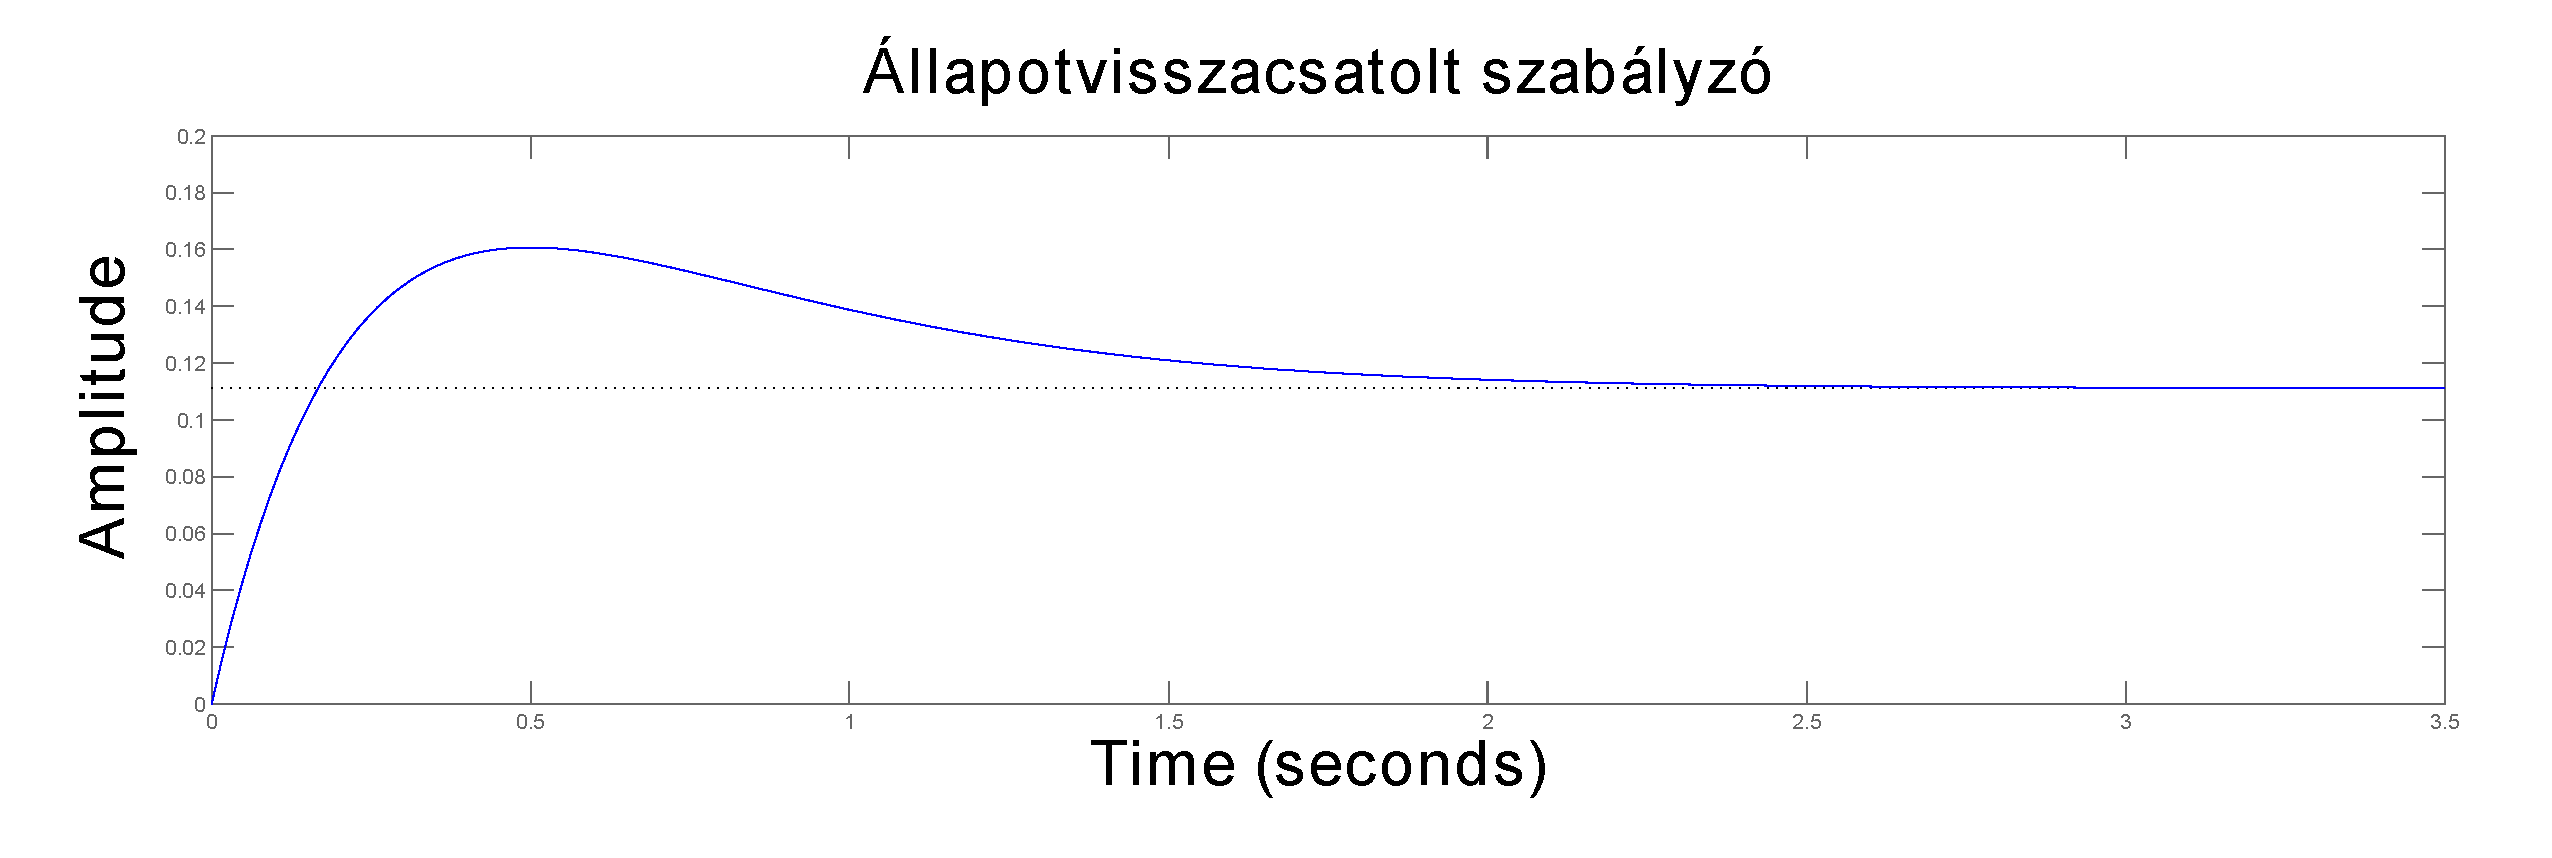
\includegraphics[width=\linewidth]{img/plot2}
    \caption{Instabil rendszer állapotvisszacsatolt stabilizációja}
    \label{fig:plot2}
\end{figure}

\paragraph{Direkt és inverz mérési modell}

A rendszer viselkedésének ismerete és egy erre létrehozott szabályzó a legritkább esetben elég a hatékony szabályzáshoz. Bizonyos állapotok csak korlátozottan, esetleg egyáltalán nem mérhetőek, így állapotmegfigyelővel kell előállítanunk. További probléma, hogy a legtöbb állapotot is csak közvetve tudjuk mérni, zajjal terhelve.
A szenzorok érzékeléseinek előállása az állapotváltozók függvényében a \textbf{Direkt mérési modell}, illetve a megfigyelhető állapotok becslése a szenzorok jelei alapján az \textbf{Inverz mérési modell}.

A kormányszabályzás esetében az optikai szenzorsorok jelei egyszerűen szimulálhatóak a rendszer állapotait és geometriai elrendezését ismervén. Az optikai szenzor mentén a vonal pozícióját a szenzorsorra való vetítéssel kaphatjuk meg:

\begin{align}
    x = \frac{d}{\cos(\delta)}
\end{align}

A direkt modell és a rendszermodell ismeretével pedig előállítható az indirekt modell is:

\begin{align}
    \hat{d} &= x \cdot \cos(\delta) \\
    \hat{c} &=\dot{x} \\
    \hat{\delta} &= \arctan \left(\frac{c}{v}\right) - \Phi
\end{align}

A direkt modell általában csak a szimuláció részét képezi, de a szenzorok jeleinek hihetőségvizsgálatát is elvégezhetjük vele futási időben, amennyiben szenzorfúziófal állítjuk elő a becsült állapotokat.
Az inverz modell az irányító rendszer legelső fokozata, a szimulációban ritkán indokolt a felhasználása.

Megjegyzendő, hogy $\delta$ közvetlenül is mérhető, ha két optikai szenzorsort helyezünk el az autón.

\subsection{Szimulációs környezet kiépítése}

A megfelelő modell és szabályzó megtervezése után elkezdhetjük a szimulációs környezetet összeállítani. Egy egyszerűbb rendszer esetében akár közvetlenül implementálni lehetne a szabályzót C-ben, ám ha a rendszer összetetteb, jobban járunk ha a modell alapú fejlesztés elvét követjük. A RobonAUT versenyre az autó irányítórendszerének implementálásához ezt az utat választottuk. A döntésben szerepet játszott a MATLAB kiváló integrált állapotgép és szimuláció támogatása, a földrajzi távolság a tesztkörnyezet (Truggy) és a lusta fejlesztő lakhelye között, illetve a technológiai kihívás vonzása is.

\paragraph{Felépítés}

A rendszert két fő logikai részre bonthatjuk, az \textbf{Irányító rendszerre} és a \textbf{Szimulátorra}, illetve egy harmadik blokk interfészt biztosít e kettő között. A MATLAB (így a Simulink is) gyengén típusos nyelv, de lehetőség van a típusok erős állítására is. Ez beágyazott rendszereknél különösen hasznos, mivel a MATLAB egészen meglepő típusokat tud előállítani magának, ami nem előnyös sem a futási sebesség, sem a kézbentarthatóság szempontjából, különösen ha fixpontos számábrázolással szeretnénk implementálni a szabályzót.

\paragraph{Szimulátor}

A megállapított rendszermodell alapján felépíthetjük a szimulátort. Hiába terveztük a szabályzót a linearizált modellhez, a szimulátornak mindig a legelső lépésben meghatározott, potenciálisan nemlineáris összefüggések alapján kell felépülnie, különben csak magunkat csapjuk be a hibás szimulációval, és az egész technológia nem ér semmit.
A nemlineáris rendszerek felépítéséhez kiváló segédletet nyújt a Szabályozástechnika tárgy 5-6. gyakorlata, illetve annak felkészülési anyaga\cite[p.~319-354]{szabtech}, így erre nem térünk ki. Amennyiben a rendszermodellt a Jacobi mátrixok segítségével generáltuk, célszerűbb közvetlenül azt felhasználni a szimulációban a blokkokból felépített rendszer helyett, így nem csak paraméter-, hanem rendszerszintű változás esetén sem kell kézzel utólag módosítani a szimulátort.

\begin{figure}[!ht]
    \centering
    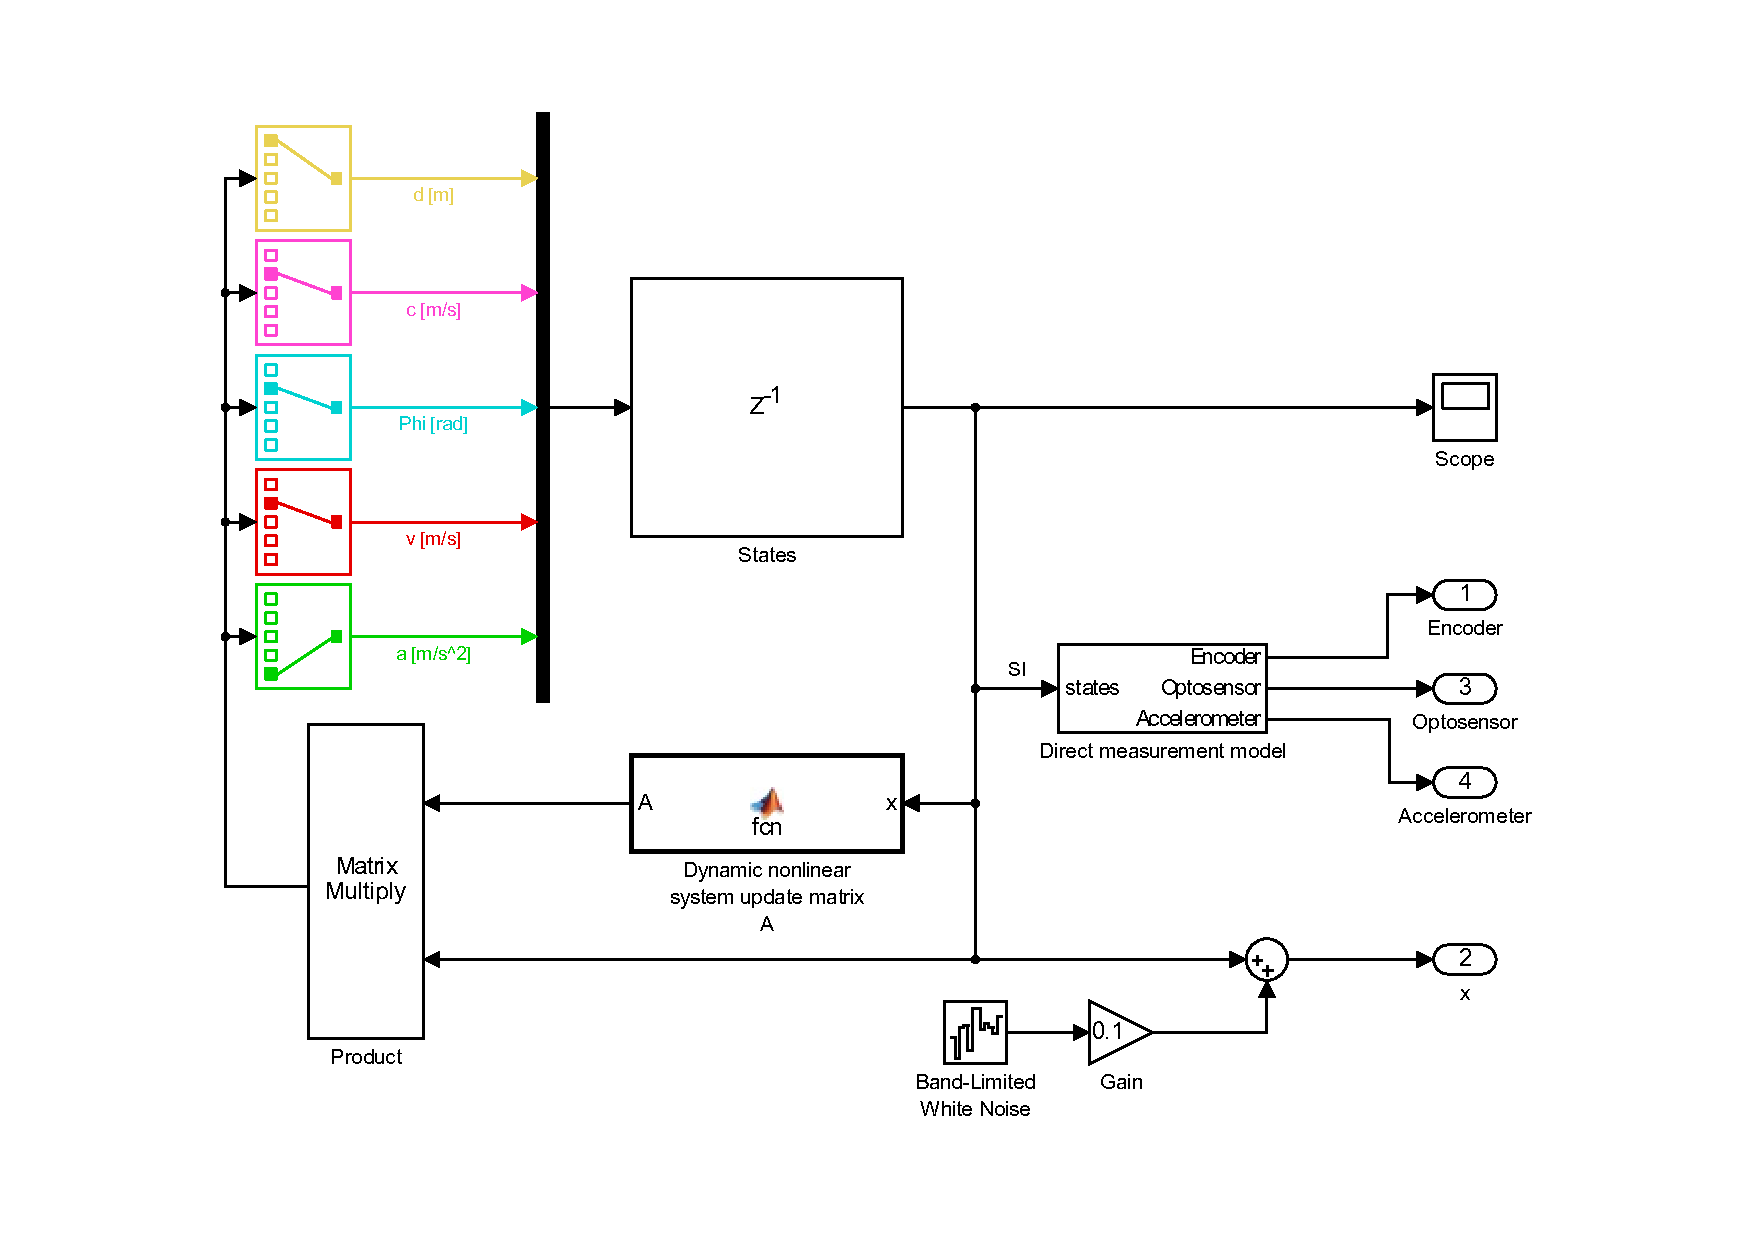
\includegraphics[width=\linewidth]{img/sys}
    \centering
    \caption{Jacobi-mátrix alapú nemlineáris szimulátor blokkdiagram}
    \label{fig:model}
\end{figure}

Ne feledjük, a szimulátor kimenete nem csupán az állapot, hanem a direkt mérési modell által előállított szimulált szenzorjelek, melyeket mesterségesen zajjal is terhelhetünk, hogy eggyel kevesebb meglepetés érjen a tényleges teszteléskor.

\subsection{Irányító rendszer implementálása}

Az irányítás tetszőlegesen bonyolult lehet, a RobonAUT-hoz készült megoldás 4 fő kritikus (működéshez elengedhetetlen) részre bontható:

\paragraph{Inverz mérési modell}

A korábban vázolt inverz mérési modell megvalósítása, célja a \textbf{visszacsatolt, mérhető állapotok} előállítása a szenzorok jelei alapján, tehát \textbf{priori információk nélkül}. Mivel a verseny során többféle jelre kellett szabályozni (vonaldetektálás, bal/jobb éldetektálás, bal/jobb távolságérzékelő szenzor jele), ezekre mind létre kell hozni az inverz mérési modellt, majd a megfelelő visszacsatolt állapotot adni tovább a jelfeldolgozónak.

\paragraph{Jelfeldolgozó és állapotbecslő}

Az inverz mérési modell által előállított \textbf{visszacsatolt állapotokat} dolgozza fel \textbf{priori információk} segítségével. Ez a mi esetünkben egy Kálmán-szűrőt jelentett, ahol a mérési jel a visszacsatolt állapot, a priori információ pedig a rendszer modellje. Bár a Kálmán-szűrő támogatja az inverz mérési modell közvetlen integrálását a szűrőbe, ezt a megoldást nem találtam célszerűnek, mivel a szenzorsor jelvektorából a vonal pozíciójele nem állítható elő zárt mátrixos alakban, valamint többféle jelentősen eltérő lehetséges bemenet között kell kapcsolni.

\paragraph{Szabályzó}

A szabályzó a szkript alapján számított paraméterek alapján implementálható, ez függ a választott szabályzó típusától és a tervezés módjától.

\paragraph{Magas szintű irányítás, állapotgép}

A magas szintű irányítás felel a szabályzás és állapotgép alapján történő vezérlés közötti kapcsolásért és a szabályzó bemeneti jelének kiválasztásáért, az aktuális állapot szerint. Ezenkívül referenciajeleket határozhat meg a sebességnek és a kormányszabályzónak.

\subsection{MATLAB Coder beállítása}

Az elkészült szabályzóból \verb!C! (vagy \verb!C++!, \verb!Verilog! és \verb!PLC!) kódot generálhatunk, melyet beágyazhatunk a rendszerbe. A generált kód egyfajta statikus osztályként működik, vannak belső tárolói és tagfüggvényei, de nem szükséges a példányosítása.

Az első lépés a kódgenerálás előkészítéséhez a megfelelő \textbf{solver} beálítása. Ezt a \textbf{Simulation/Configuration parameters... (Ctrl + E)} menüpontban tehetjük meg a \textbf{Solver} menüpontban. A típust Fixed-step-re kell állítani, a solvert pedig discrete-re, hogy egyáltalán nem legyenek folytonos állapotok a modellünkben. Ezután ne felejtsük el megadni a mintavételi idejét a rendszernek, másodpercben.
Ezt a beállítást célszerű már a modell létrehozásakor, a legelső lépésként elvégezni, ugyanis egy folytonos környezetben épített modell nem feltétlenül fog működni diszkrét solverrel! (Alternatív módon \textbf{Atomic Subsystem} blokkba helyezhetjük a fordítani kívánt rendszert, amennyiben mindenképpen folytonos idejű szimulátorral szeretnénk dolgozni. Ekkor nem szükséges a solver módosítása, viszont gondoskodni kell a mintavételi idő váltásról.)

A tényleges kódgeneráláshoz szükség van egy MATLAB által támogatott \verb!C/C++! compilerre is. A teljes lista megtekinthető a MathWorks weboldalán.\footnote{http://www.mathworks.com/support/compilers/}

\paragraph{Target beállítása}

A kódgenerálásra millióféle különböző beállítás létezik, ezek közül az STM32F4-Discovery kártyához tartozót mutatjuk be, mivel ez volt a célplatform a RobonAUT verseny során.

A \textbf{Hardware Implementation} menüpontban a \textbf{Device Vendor} legördülő listát állítsuk \textbf{ARM Compatible}-re, a \textbf{Device type}-ot pedig \textbf{ARM Cortex}-re.
A \textbf{Code Generation} menüpontban állítsuk át a \textbf{System target file}-t \textbf{ert.tlc}-re (ezzel az általános MATLAB-Embedded codert hívjuk meg).
Az \textbf{Interface} menüpontban a \textbf{Code Replacement Library}-t állítsuk \textbf{GCC ARM Cortex-M3}-re.
Amennyiben lebegőpontos számábrázolást is használunk a programban, kapcsoljuk be ezeknek a támogatását. Kihasználatlanul viszont nem javasolt mindent bekapcsolni, mivel csak felesleges típusdefiníciók jönnek létre. Ha valamit elfelejtettünk beállítani, Build közben hibajelzéssel ide fog visszairányítani a MATLAB.
A \textbf{Report} menüpontban bekapcsolható a "Create code generation report", ami egy dokumentációt is generál a kód mellé.
A \textbf{Code Generation} menüponthoz visszatérve bekapcsolhatjuk az optimalizációkat is, így javíthatunk a kód futásteljesítményén, valamint a generálás sebességén növelhetjük, ha nem kérünk make-filet, illetve buildet egyből, hanem csak a kódot állítjuk elő (úgyis csak arra van szükségünk itt).
A kezelhetőséget javítja, ha a \textbf{Code placement}-ben a \textbf{Code packaging}-et \textbf{Compact}-ra állítjuk, így kevesebb forrásfájlt generál, és könnyebb kezelni, ha csak egy generált rendszerünk van.

\paragraph{Tl;dr}

\begin{itemize}

    \item \textbf{Solver} $\rightarrow$ Fixed step, discrete
    \item \textbf{Hardware Implementation} $\rightarrow$ Device type $\rightarrow$ ARM Cortex
    \item \textbf{Code Generation} $\rightarrow$ System Target File $\rightarrow$ ert.tlc
    \item \textbf{Interface} $\rightarrow$ Code Replacement Library $\rightarrow$ GCC ARM Cortex-M3
    \item \textbf{MATLAB Command Line} $\rightarrow$ \textbf{mex -setup}

\end{itemize}

\subsection{Kódgenerálás}

A megfelelő beállítás után a Simulink modellben keressük meg azt a blokkot, melyből kódot szeretnénk generálni. Egy nagy rendszerben akár több részben is lehet kódot generálni, pl. kapcsolható működés, vagy eltérő mintavételi idő esetén hasznos. Jelen esetben az Irányító rendszer blokkját szeretnénk felhasználni, melynek bemenete a szenzoroktól kapott közvetlen jel, kimenete pedig a szervójel. A blokkon jobb kattintás, majd \textbf{C/C++ Code} $\rightarrow$ \textbf{Build This Subsystem} (Régebbi MATLAB verziókban MATLAB Coder, illetve Real Time Workshop (RTW) menüpontokat kell keresni). A generált fileok a \verb!MATLAB Current Working Folder!-be kerülnek, nem a generált rendszer mellé.









